\documentclass[8pt,a4paper,compress,handout]{beamer}

\usepackage{/home/siyer/lib/slides}

\title{Case Study: Percolation Problem}
\date{}

\begin{document}
\begin{frame}
\hfill
\begin{minipage}{150pt}
\begin{flushright}
\tiny \emph{Where is everybody?}

\smallskip

- ENRICO FERMI
\end{flushright}
\end{minipage}
\vfill
\titlepage
\end{frame}

\begin{frame}
\frametitle{Outline}
\tableofcontents
\end{frame}

\section{Percolation}
\begin{frame}[fragile]
Pour liquid on top of some porous material. Will the liquid reach the bottom? 

\bigskip

\emph{Percolation} refers to the abstract process that models such situations.

\bigskip

Some Applications:
\begin{itemize}
\item Spread of forest fires.
\item Flow of electricity through a network of resistors.
\item Permeation of gas in a coal mine through a gas mask filter.
\item Studying \emph{Fermi's paradox}, the apparent contradiction between the high estimates of the probability of the existence of extraterrestrial civilizations and the lack of evidence for them.
\end{itemize}
\end{frame}

\begin{frame}[fragile]
Abstract model:
\begin{itemize}
\item $n$-by-$n$ grid of sites.
\item Each site is either \emph{blocked} or \emph{open}.
\item An open site is \emph{full} if it is connected to the top via open sites.
\end{itemize}

\begin{center}
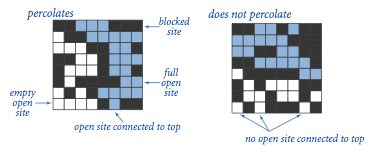
\includegraphics[scale=0.4]{figures/percolation1.png}

\smallskip

\tiny Percolation model
\end{center}

\bigskip

If sites are independently set to be open with vacancy probability $p$, what is the probability that the system percolates?

\bigskip

There is no known mathematical solution, so we take a computational (Monte Carlo simulation) approach.

\bigskip

We use one $n$-by-$n$ boolean matrix to store which sites are open, and another to compute which sites are full. 
\end{frame}

\begin{frame}[fragile]
\begin{framed}
\tiny percolationio.py: Implements percolation support functions.
\end{framed}

\begin{lstlisting}[language=Python]
import stdarray
import stddraw
import stdrandom
import sys

def random(n, p):
    a = stdarray.create2D(n, n, False)
    for i in range(n):
        for j in range(n):
            a[i][j] = stdrandom.bernoulli(p)
    return a

def draw(a, which):
    n = len(a)
    stddraw.setXscale(-.5, n)
    stddraw.setYscale(-.5, n)
    for i in range(n):
        for j in range(n):
            if a[i][j] == which:
                stddraw.filledSquare(j, n - i - 1, .5)

def main():
    n = int(sys.argv[1])
    p = float(sys.argv[2])
    test = random(n, p)
    draw(test, False)
    stddraw.show()
    
if __name__ == '__main__':
    main()
\end{lstlisting}
\end{frame}

\begin{frame}[fragile]
\begin{minipage}{160pt}
\begin{lstlisting}[language={}]
$ python percolationio.py 10 .8
\end{lstlisting}
\end{minipage}%
\begin{minipage}{140pt}
\hfill 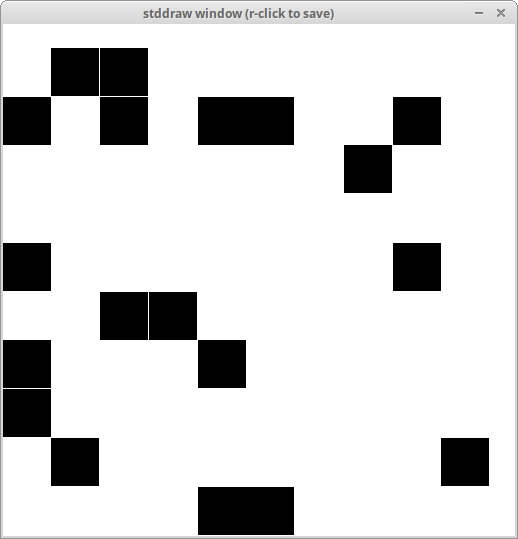
\includegraphics[scale=0.15]{figures/percolation2.png}
\end{minipage}

\smallskip

\begin{minipage}{160pt}
\begin{lstlisting}[language={}]
$ python percolationio.py 10 .2
\end{lstlisting}
\end{minipage}%
\begin{minipage}{140pt}
\hfill 
\includegraphics[scale=0.15]{figures/percolation3.png}
\end{minipage}

\smallskip

\begin{minipage}{160pt}
\begin{lstlisting}[language={}]
$ python percolationio.py 100 .6
\end{lstlisting}
\end{minipage}%
\begin{minipage}{140pt}
\hfill 
\includegraphics[scale=0.15]{figures/percolation4.png}
\end{minipage}
\end{frame}

\section{Vertical Percolation}
\begin{frame}[fragile]
We start by solving an easier version of the problem, namely \emph{vertical percolation}: Is there a path of open sites from the top to the bottom that goes \emph{straight down}?

\begin{center}
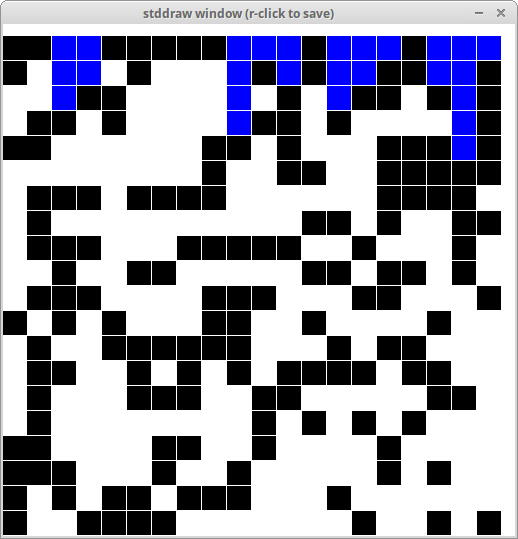
\includegraphics[scale=0.4]{figures/percolation5.png}

\smallskip

\tiny Vertical percolation
\end{center}

\bigskip

A site $(i, j)$ is full if it is open \emph{and} site $(i-1, j)$ is full.

\bigskip

To determine if a system vertically percolates, scan rows from top to bottom.

\begin{center}
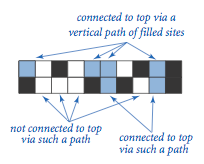
\includegraphics[scale=0.4]{figures/percolation6.png}

\smallskip

\tiny Vertical percolation testing
\end{center}
\end{frame}

\begin{frame}[fragile]
\begin{framed}
\tiny percolationv.py: Read from standard input a boolean matrix that represents the open sites of a system. Write to standard output a boolean matrix representing the full sites of the system. Then write \lstinline{True} if the system percolates and \lstinline{False} otherwise.
\end{framed}

\begin{lstlisting}[language=Python]
import stdarray
import stdio

def flow(isOpen):
    n = len(isOpen)
    isFull = stdarray.create2D(n, n, False)
    for j in range(n):
        isFull[0][j] = isOpen[0][j]
    for i in range(1, n):
        for j in range(n):
            if isOpen[i][j] and isFull[i - 1][j]:
                isFull[i][j] = True
    return isFull

def percolates(isOpen):
    isFull = flow(isOpen)
    n = len(isFull)
    for j in range(n):
        if isFull[n - 1][j]:
            return True
    return False

def main():
    isOpen = stdarray.readBool2D()
    stdarray.write2D(flow(isOpen))
    stdio.writeln(percolates(isOpen))
    
if __name__ == '__main__':
    main()
\end{lstlisting}
\end{frame}

\begin{frame}[fragile]
\begin{lstlisting}[language={}]
$ more test8.txt 
8 8
0 0 1 1 1 0 0 0
1 0 0 1 1 1 1 1
1 1 1 0 0 1 1 0
0 0 1 1 0 1 1 1
0 1 1 1 0 1 1 0
0 1 0 0 0 0 1 1
1 0 1 0 1 1 1 1
1 1 1 1 0 1 0 0
$ python percolationv.py < test8.txt 
8 8
0 0 1 1 1 0 0 0 
0 0 0 1 1 0 0 0 
0 0 0 0 0 0 0 0 
0 0 0 0 0 0 0 0 
0 0 0 0 0 0 0 0 
0 0 0 0 0 0 0 0 
0 0 0 0 0 0 0 0 
0 0 0 0 0 0 0 0 
False
\end{lstlisting}
\end{frame}

\begin{frame}[fragile]
\begin{framed}
\tiny visualizev.py: Accept integer $n$, float $p$, and integer $trials$ as command-line arguments. Generate an $n$-by-$n$ random system with site vacancy probability $p$. Compute the directed percolation flow, and draw result to standard draw. Repeat $trials$ times.
\end{framed}

\begin{lstlisting}[language=Python]
import percolationio
import percolationv
import stddraw
import sys

def main():
    n = int(sys.argv[1])
    p = float(sys.argv[2])
    trials = int(sys.argv[3])
    for i in range(trials):
        isOpen = percolationio.random(n, p)
        stddraw.clear()
        stddraw.setPenColor(stddraw.BLACK)
        percolationio.draw(isOpen, False)
        stddraw.setPenColor(stddraw.BLUE)
        full = percolationv.flow(isOpen)
        percolationio.draw(full, True)
        stddraw.show(1000.0)
    stddraw.show()

if __name__ == '__main__':
    main()
\end{lstlisting}
\end{frame}

\begin{frame}[fragile]
\begin{minipage}{160pt}
\begin{lstlisting}[language={}]
$ python visualizev.py 20 .65 1
\end{lstlisting}
\end{minipage}%
\begin{minipage}{140pt}
\hfill 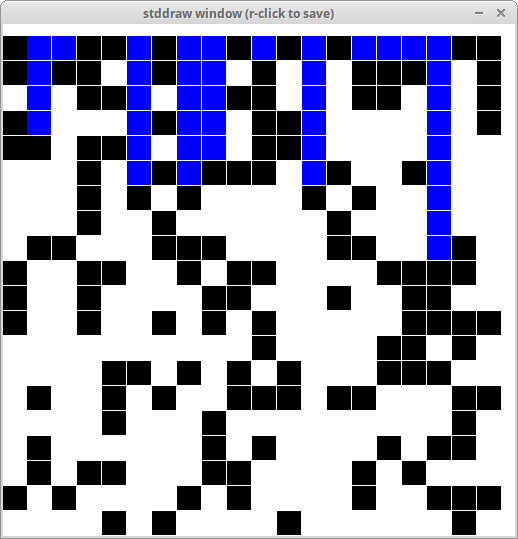
\includegraphics[scale=0.15]{figures/percolation7.png}
\end{minipage}

\smallskip

\begin{minipage}{160pt}
\begin{lstlisting}[language={}]
$ python visualizev.py 20 .60 1
\end{lstlisting}
\end{minipage}%
\begin{minipage}{140pt}
\hfill 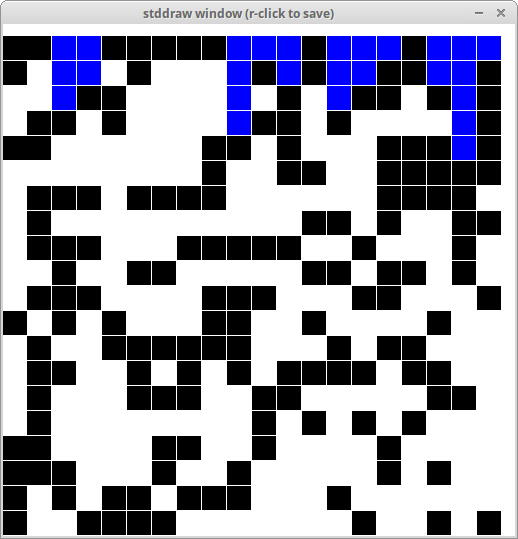
\includegraphics[scale=0.15]{figures/percolation8.png}
\end{minipage}

\smallskip

\begin{minipage}{160pt}
\begin{lstlisting}[language={}]
$ python visualizev.py 20 .55 1
\end{lstlisting}
\end{minipage}%
\begin{minipage}{140pt}
\hfill 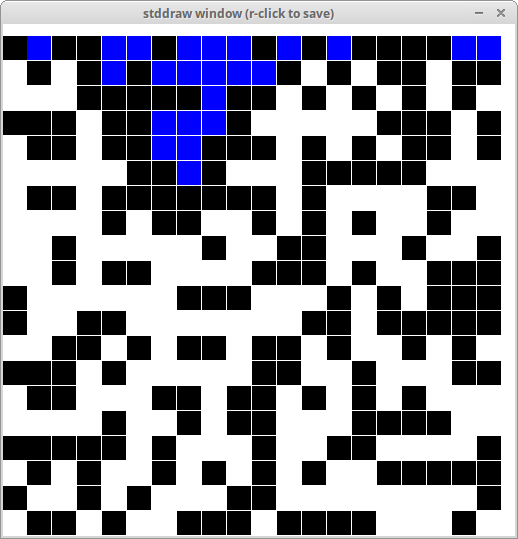
\includegraphics[scale=0.15]{figures/percolation9.png}
\end{minipage}
\end{frame}

\begin{frame}[fragile]
\begin{framed}
\tiny estimatev.py: Accept integer $n$, float $p$, and integer $trials$ as command-line arguments. Create $trials$ random $n$-by-$n$ systems with site vacancy probability $p$. Determine the fraction of them that percolate, and
write that fraction to standard output.
\end{framed}

\begin{lstlisting}[language=Python]
import percolationio
import percolationv
import stdio
import sys

def evaluate(n, p, trials):
    count = 0
    for i in range(trials):
        isOpen = percolationio.random(n, p)
        if (percolationv.percolates(isOpen)):
            count += 1
    return 1.0 * count / trials

def main():
    n = int(sys.argv[1])
    p = float(sys.argv[2])
    trials = int(sys.argv[3])
    q = evaluate(n, p, trials)
    stdio.writeln(q)
    
if __name__ == '__main__': 
    main()
\end{lstlisting}

\begin{lstlisting}[language={}]
$ python estimatev.py 20 .65 1000
0.004
$ python estimatev.py 20 .60 1000
0.001
$ python estimatev.py 20 .55 1000
0.0
\end{lstlisting}
\end{frame}

\section{General Percolation}
\begin{frame}[fragile]
Given an $n$-by-$n$ system, is there \emph{any} path of open sites from the top to the bottom?

\bigskip

To visit all sites reachable from site $(i, j)$, do \emph{depth first search (DFS)}:
\begin{itemize}
\item If $(i, j)$ already marked as reachable, return.
\item If $(i, j)$ not open, return.
\item Mark $(i, j)$ as reachable.
\item Visit the four neighbors of $(i, j)$ recursively.
\end{itemize}

\bigskip

Percolation solution:
\begin{itemize}
\item Run DFS from each site of top row.
\item Check if any site in bottom row is marked as reachable.
\end{itemize}
\end{frame}

\begin{frame}[fragile]
\begin{framed}
\tiny percolation.py: Read from standard input a boolean matrix that represents the open sites of a system. Write to standard output a boolean
matrix representing the full sites of the system. Then write \lstinline{True} if the system percolates and \lstinline{False} otherwise.

\end{framed}

\begin{lstlisting}[language=Python]
import stdarray
import stdio

def _flow(isOpen, isFull, i, j):
    n = len(isFull)
    if (i < 0) or (i >= n):
        return
    if (j < 0) or (j >= n):
        return
    if not isOpen[i][j]:
        return
    if isFull[i][j]:
        return
    isFull[i][j] = True
    _flow(isOpen, isFull, i + 1, j)
    _flow(isOpen, isFull, i, j + 1)
    _flow(isOpen, isFull, i, j - 1)
    _flow(isOpen, isFull, i - 1, j)

def flow(isOpen):
    n = len(isOpen)
    isFull = stdarray.create2D(n, n, False)
    for j in range(n):
        _flow(isOpen, isFull, 0, j)
    return isFull
\end{lstlisting}
\end{frame}

\begin{frame}[fragile]
\begin{lstlisting}[language=Python]
def percolates(isOpen):
    isFull = flow(isOpen)
    n = len(isFull)
    for j in range(n):
        if isFull[n - 1][j]:
            return True
    return False

def main():
    isOpen = stdarray.readBool2D()
    stdarray.write2D(flow(isOpen))
    stdio.writeln(percolates(isOpen))

if __name__ == '__main__':
    main()
\end{lstlisting}
\end{frame}

\begin{frame}[fragile]
\begin{lstlisting}[language={}]
$ more test8.txt 
8 8
0 0 1 1 1 0 0 0
1 0 0 1 1 1 1 1
1 1 1 0 0 1 1 0
0 0 1 1 0 1 1 1
0 1 1 1 0 1 1 0
0 1 0 0 0 0 1 1
1 0 1 0 1 1 1 1
1 1 1 1 0 1 0 0
$ python percolation.py < test8.txt 
8 8
0 0 1 1 1 0 0 0 
0 0 0 1 1 1 1 1 
0 0 0 0 0 1 1 0 
0 0 0 0 0 1 1 1 
0 0 0 0 0 1 1 0 
0 0 0 0 0 0 1 1 
0 0 0 0 1 1 1 1 
0 0 0 0 0 1 0 0 
True
\end{lstlisting}
\end{frame}

\begin{frame}[fragile]
\begin{framed}
\tiny visualize.py: Accept integer $n$, float $p$, and integer $trials$ as command-line arguments. Generate an $n$-by-$n$ random system with site vacancy probability $p$. Compute the directed percolation flow, and draw result to standard draw. Repeat $trials$ times.
\end{framed}

\begin{lstlisting}[language=Python]
import percolation
import percolationio
import stddraw
import sys

def main():
    n = int(sys.argv[1])
    p = float(sys.argv[2])
    trials = int(sys.argv[3])
    for i in range(trials):
        isOpen = percolationio.random(n, p)
        stddraw.clear()
        stddraw.setPenColor(stddraw.BLACK)
        percolationio.draw(isOpen, False)
        stddraw.setPenColor(stddraw.BLUE)
        full = percolation.flow(isOpen)
        percolationio.draw(full, True)
        stddraw.show(1000.0)
    stddraw.show()

if __name__ == '__main__':
    main()
\end{lstlisting}
\end{frame}

\begin{frame}[fragile]
\begin{minipage}{160pt}
\begin{lstlisting}[language={}]
$ python visualize.py 20 .65 1
\end{lstlisting}
\end{minipage}%
\begin{minipage}{140pt}
\hfill 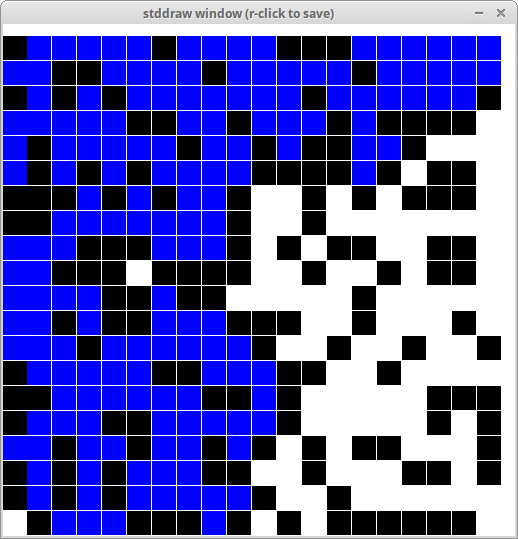
\includegraphics[scale=0.15]{figures/percolation10.png}
\end{minipage}

\smallskip

\begin{minipage}{160pt}
\begin{lstlisting}[language={}]
$ python visualize.py 20 .60 1
\end{lstlisting}
\end{minipage}%
\begin{minipage}{140pt}
\hfill 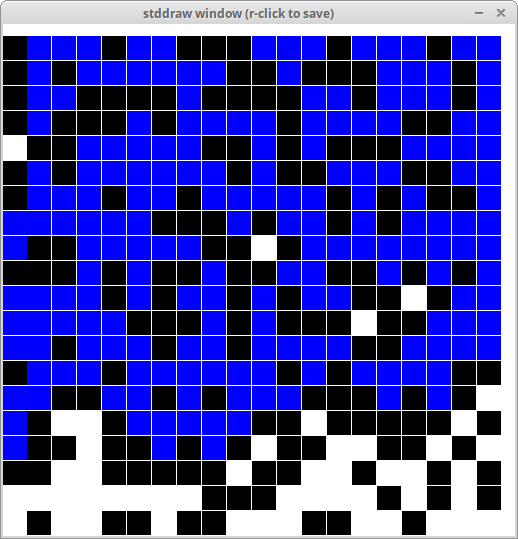
\includegraphics[scale=0.15]{figures/percolation11.png}
\end{minipage}

\smallskip

\begin{minipage}{160pt}
\begin{lstlisting}[language={}]
$ python visualize.py 20 .55 1
\end{lstlisting}
\end{minipage}%
\begin{minipage}{140pt}
\hfill 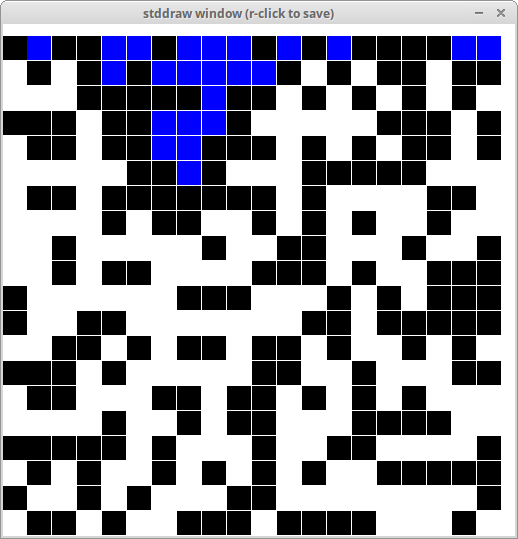
\includegraphics[scale=0.15]{figures/percolation12.png}
\end{minipage}
\end{frame}

\begin{frame}[fragile]
\begin{framed}
\tiny estimate.py: Accept integer $n$, float $p$, and integer $trials$ as command-line arguments. Create $trials$ random $n$-by-$n$ systems with site vacancy probability $p$. Determine the fraction of them that percolate, and
write that fraction to standard output.
\end{framed}

\begin{lstlisting}[language=Python]
import percolation
import percolationio
import stdio
import sys

def evaluate(n, p, trials):
    count = 0
    for i in range(trials):
        isOpen = percolationio.random(n, p)
        if (percolation.percolates(isOpen)):
            count += 1
    return 1.0 * count / trials

def main():
    n = int(sys.argv[1])
    p = float(sys.argv[2])
    trials = int(sys.argv[3])
    q = evaluate(n, p, trials)
    stdio.writeln(q)

if __name__ == '__main__':
    main()
\end{lstlisting}

\begin{lstlisting}[language={}]
$ python estimate.py 20 .65 1000
0.868
$ python estimate.py 20 .60 1000
0.557
$ python estimate.py 20 .55 1000
0.222
\end{lstlisting}
\end{frame}
\end{document}
